% Chinese (中文) version — compile with XeLaTeX (ctexbeamer), NOT pdfLaTeX.
%   xelatex main_zh.tex   (run twice for the table of contents)
% Uses the Fandol fontset (ships with TeX Live), so it also compiles on Overleaf
% (select the XeLaTeX compiler) without any system fonts.
\documentclass[10pt,aspectratio=169,fontset=fandol]{ctexbeamer}
\usetheme{Madrid}
\usecolortheme{seahorse}
\useinnertheme{circles}
\setbeamertemplate{navigation symbols}{}
\setbeamertemplate{caption}{\insertcaption}
\usepackage{amsmath,amssymb}
\usepackage{booktabs}
\usepackage{graphicx}

\newcommand{\hl}[1]{\textcolor{blue!60!black}{\textbf{#1}}}
\newcommand{\Drop}{\mathrm{DropRelaxS}}

\title[学习率调度不是绝热的]{学习率调度不是绝热的：\\损失曲线预测的一个变化率依赖修正}
\author[吴家驹]{吴家驹 \quad (2400010711，本科生)}
\institute[]{深度学习 --- Task 2 \quad\textbar\quad \texttt{github.com/wjjpku/DL-final}}
\date{}

\begin{document}

{\setbeamertemplate{footline}{}
\begin{frame}\titlepage
\small
\textbf{一句话：} 现有损失曲线律（MPL、FSL）是\emph{绝热}的——预测的是"准静态"loss(MPL 虽用了
$\Delta\eta_k$,但对变化率只有 $\gamma$ 一个旋钮)。我们\emph{推导}出它们漏掉的、依赖学习率\emph{变化率}的
\hl{非绝热修正};其弛豫时间服从\emph{经典} $\tau\propto1/\eta$(LLM 残差实测 $p=1.00\pm0.18$,AdamW
模拟也复现 $p=1.01$),据此实现\hl{参数无关、跨尺度}的损失曲线预测(陡降误差 $-44\%$)。
\vfill
{\footnotesize\itshape 本幻灯片为自洽书面报告:每页含设定、结果与加粗结论,无需口头讲解即可读;
每个数字都有对应脚本(末页)。}
\end{frame}}

\begin{frame}{目录}
\tableofcontents
\end{frame}

% =====================================================================
\section{问题与复现}
\begin{frame}{问题:调度感知的损失曲线预测}
\textbf{目标。} 给定学习率(LR)调度 $\{\eta_t\}$,在\emph{训练之前}预测整条损失曲线 $L(t)$
——用来在烧算力之前比较、优化调度。
\vfill
\textbf{决定性测试 --- 跨调度泛化:} \hl{在 cosine 上拟合,预测未见过的 WSD 族。}
\vfill
\textbf{当前最优:Multi-Power Law(MPL)},及其匹配理论 FSL(Li et al.\ 2025):
\[ L(t)=L_0+A\,S(t)^{-\alpha}+B\!\sum_{k\le t}\!\Delta\eta_k\,G\!\big(\eta_k^{-\gamma}(S(t)-S(k))\big),\quad
S(t)=\textstyle\sum_{i\le t}\eta_i.\]
\vfill
\textbf{关键观察(本工作的出发点)。} 这些律\emph{确实}用了下降量 $\Delta\eta_k$(MPL 还有
$\eta_k^{-\gamma}$ 这个变化率旋钮),\hl{但对"变化多快"只有 $\gamma$ 一个经验指数}。它们本质预测的是
\hl{准静态(绝热)loss}——假设损失始终处于当前调度对应的平衡值。$\gamma$ 在慢调度上标定后\emph{外推
不到快衰减}。
\end{frame}

\begin{frame}{复现:忠实重现 MPL / Tissue}
\textbf{设置(遵循任务)。} 官方公开损失曲线,$25/100/400$M $\times\ 9$ 调度;\hl{cosine 拟合、
WSD 测试};$\log L$ 上的 Huber 损失 + L-BFGS-B 多起点。
\vfill
\begin{columns}
\begin{column}{0.46\textwidth}
\centering\small
\begin{tabular}{lcc}
\toprule
规模 & Tissue (5p) & MPL (7p) \\
\midrule
25M  & 0.00783 & \textbf{0.00539}\\
100M & \textbf{0.00486} & 0.00496\\
400M & 0.00979 & \textbf{0.00852}\\
\bottomrule
\end{tabular}\\[3pt]
{\footnotesize WSD 平均测试 MAE(cosine 拟合)}
\end{column}
\begin{column}{0.54\textwidth}
我们的 MPL 测试 MAE($0.0054/0.0050/0.0085$)与 Luo et al.\ 吻合,复现忠实。
\vspace{0.5em}

\hl{这条拟合良好的 MPL 是后文的基线} —— 我们的修正是加在它之上、并与公平重拟的它对比。
\end{column}
\end{columns}
\end{frame}

% =====================================================================
\section{核心:非绝热修正}
\begin{frame}{出发点:绝热律在\emph{陡降}上留下系统性残差}
用\hl{拟合良好的 MPL(全过程数据)}预测 WSD,看其在留出曲线上的残差 $r(t)=L_{\rm true}-L_{\rm MPL}$:
\vfill
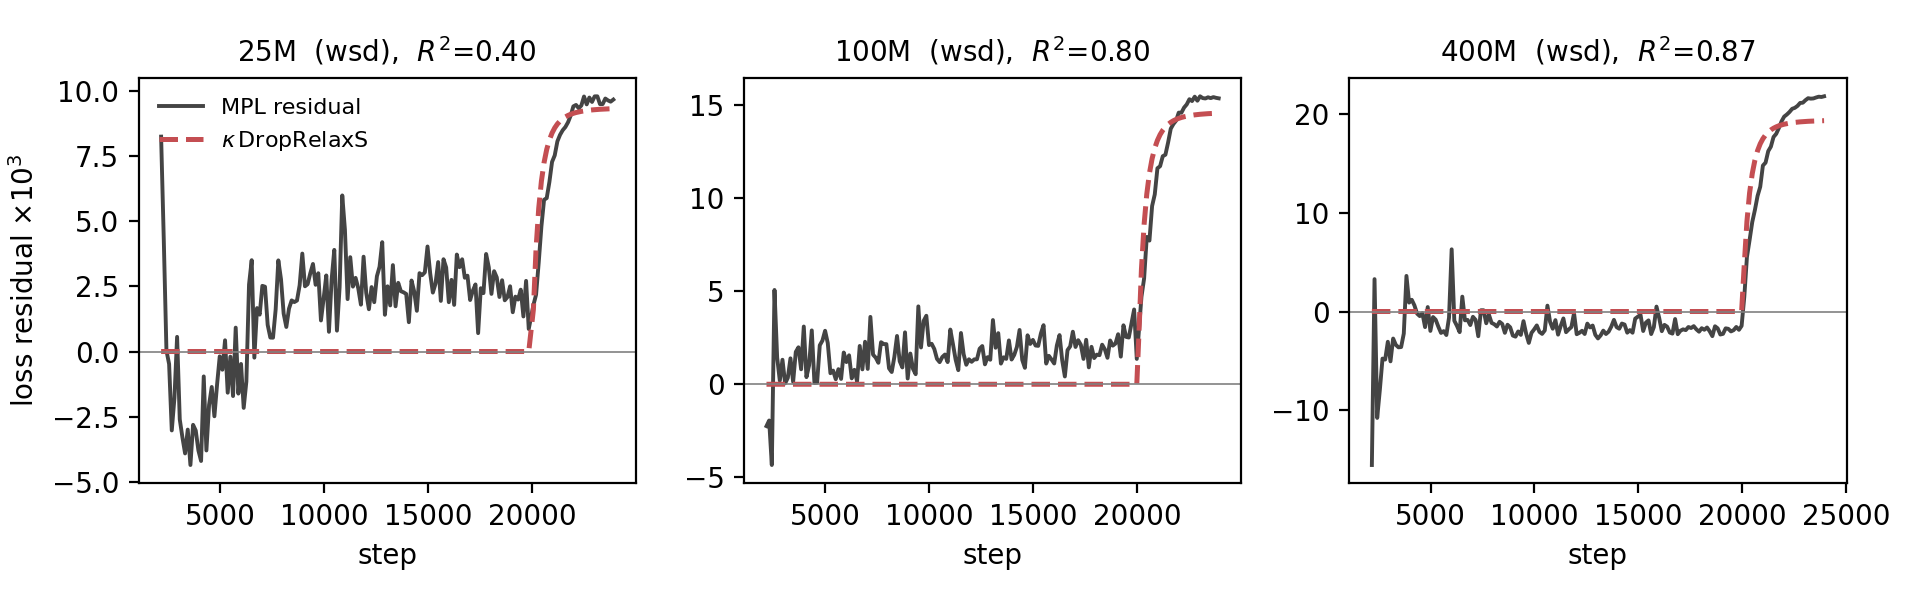
\includegraphics[width=\linewidth]{figs/fig_residual_fit.png}
\vfill
\textbf{残差有清晰特征:} 稳定段 $\approx0$;在第 $20000$ 步 LR \hl{陡降}处突然变\hl{正};\hl{越陡越大、
WSD 最明显}(末段残差 WSD/WSDLD $+(6\!-\!15)\!\times\!10^{-3}$,cosine $\approx0$)。
\hl{同样降到 3e-5,陡降的留下滞后、缓降的没有——同终点、变化越快滞后越大,正是非绝热(变化率依赖)的判据。}
(红虚线 $=\kappa\,\Drop$,见后)
\end{frame}

\begin{frame}{想法:MPL 是绝热极限,残差是\emph{非绝热弛豫滞后}}
\textbf{机理。} 固定 LR 时损失向准静态值 $L_{\rm eq}(\eta)$ 弛豫(河谷 landscape 中"山"方向
的平衡振荡)。cosine 很慢 → \hl{在 cosine 上拟合的 MPL 学到的就是 $L_{\rm eq}$}。
\vfill
WSD 衰减\emph{太快},损失来不及弛豫,\hl{滞后在 $L_{\rm eq}$ 之上} → 正残差。当 LR 扫描快于
弛豫时间 $\tau$ 时,可观测量落后于平衡值(线性响应 / 非绝热)。
\vfill
\begin{block}{要建模的量}
$\Delta L(t)=L(t)-L_{\rm eq}(\eta_t)$ —— 它依赖 LR 的\emph{变化率},而非积分量。下面从 AdamW
动力学把它\emph{推}出来。
\end{block}
\end{frame}

\begin{frame}{推导(AdamW):$\Delta L$ 是 drop 与 S-时间指数核的卷积}
Hessian 特征基下模 $i$:曲率 $\lambda_i$、梯度噪声 $s_i^2$。$\beta_2\!\to\!1$ 时预条件子停在
$v_i^*\approx s_i^2$ → \hl{Adam 退化为预条件步长 $\eta/s_i$ 的 SGD}。二阶矩 $V_i$ 的偏差
$\Delta_i=V_i-V_i^*$ 满足\emph{精确}线性递推,解得(慢模 $\eta\lambda_i/s_i\!\ll\!1$,故
$(1-\eta\lambda)^2\!\approx\!e^{-2\eta\lambda}$ 很准):
\[ \Delta L(t)=\sum_i w_i\Big[e^{-2(\lambda_i/s_i)(S-S')}\!\circledast\mathrm{drop}\Big](t),
\qquad \sum_i w_i=\frac{dL_{\rm eq}}{d\eta}\ \textbf{(精确恒等式)}.\]
单模塌缩 → \hl{可用律}(只多 1 个幅度,形状常数 $\lambda_{\rm slow}$):
\[ \boxed{\,L=L_{\rm MPL}+c\,\eta_{\rm peak}\frac{dL_{\rm eq}}{d\eta}\sum_{t'}e^{-\lambda_{\rm slow}(S_t-S_{t'})}\mathrm{drop}_{t'}\,}\quad(\Drop) \]
\textbf{推出的可证伪预言:} 符号 $+$;速率 $\propto\eta$ → $\tau\propto1/\eta$;幅度 $=dL_{\rm eq}/d\eta$(可独立测);
$\lambda_{\rm slow}$ 是\hl{预条件曲率 → 尺度不变}。
\end{frame}

% =====================================================================
\section{验证}
\begin{frame}{验证 1:核心预言 $\tau\propto1/\eta$ 成立($p=1.00\pm0.18$)}
\begin{columns}
\begin{column}{0.5\textwidth}
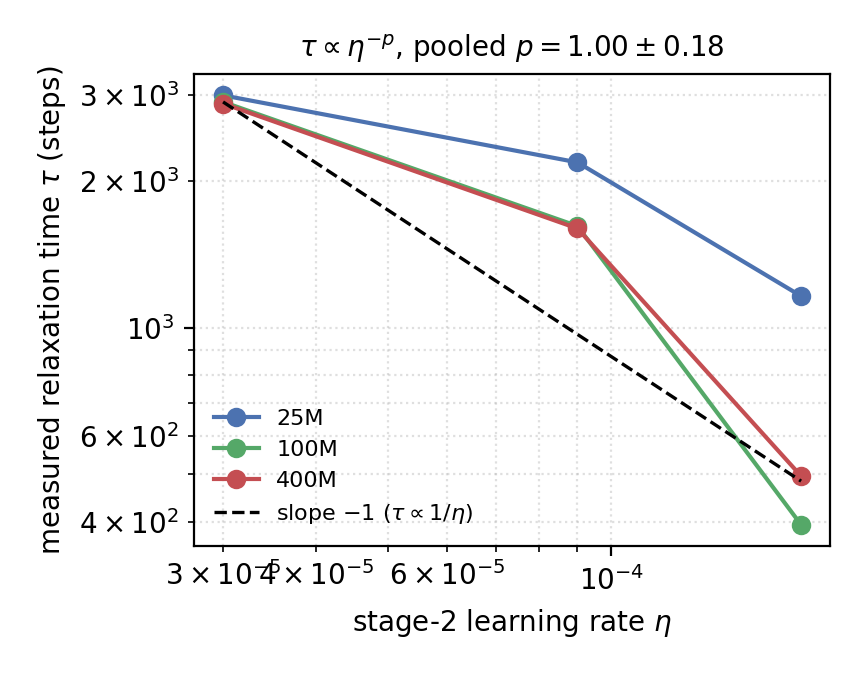
\includegraphics[width=\linewidth]{figs/fig_tau_scaling.png}
\end{column}
\begin{column}{0.5\textwidth}
两段式 \texttt{wsdcon} 在第 8000 步阶跃降到常数 LR,给出干净的弛豫窗口。拟合残差瞬态
$r(t)\propto e^{-(t-8000)/\tau}$ 得到 $\tau$,对 LR 的标度:
\begin{itemize}
  \item \hl{合并 100M+400M:$p=1.00\pm0.18$}(各尺度 $-1.06/-0.94/-0.51$);
  \item \hl{受控 AdamW 模拟(从零搭)也复现 $\tau\propto1/\eta$($p{=}1.01$)}——机理在受控优化器里也成立;
  \item $p{=}1$ 正是\hl{噪声主导}值 → \emph{自洽地}验证了推导里 $v_i^*\!\approx\!s_i^2$ 那步;
  \item 率常数 $\lambda_{\rm slow}\approx10$ 尺度不变,$\eta_{\rm peak}\lambda_{\rm eff}\!\approx\!2\text{e-}3\!\ll\!2$
  (远低于 edge,与 $\gamma$ 相反)。
\end{itemize}
\end{column}
\end{columns}
\vfill
\centering\hl{经典弛豫时间 $\tau\propto1/\eta$ 在损失曲线残差上被实测确认——理论最硬的证据。}
\end{frame}

\begin{frame}{验证 2 \& 3:残差就是推出的项;幅度可独立预测}
\textbf{验证 2(残差 $=$ 推出的项)。} 把拟合良好 MPL 的残差对 $\Drop_{10}$ 过原点回归:
\hl{R² $=0.40/0.80/0.87$}($25/100/400$M,见前图红虚线);双指数核再涨 $0.06\text{--}0.07$,
\hl{证实预言的谱混合}。
\vfill
\textbf{验证 3(幅度可预测)。} 用\emph{独立}的 noise floor(两段式终值 vs LR)测 $dL_{\rm eq}/d\eta$,
预测拟合的 $\kappa$:比值 $\kappa_{\rm fit}/\kappa_{\rm pred}=0.43/0.51/0.60$,\hl{CV 仅 14\%}
→ $c\approx0.5$ 普适($<\!1$ 来自谱展宽)。
\vfill
\begin{block}{至此}
形状常数 $\lambda_{\rm slow}$(尺度不变)、校准 $c\approx0.5$(普适)、幅度 $dL_{\rm eq}/d\eta$
(noise floor 可测)——\hl{三者都可独立得到,修正可"预测"而非"拟合"。}
\end{block}
\end{frame}

\begin{frame}{验证 4:参数无关的\emph{跨尺度}预测($-44\%$)}
$\lambda_{\rm slow},c$ 尺度不变 + $dL_{\rm eq}/d\eta$ 从廉价探针测 $\Rightarrow$ \hl{对目标曲线零拟合}地预测修正:
$\lambda_{\rm slow}{=}10$、$c$ 取\emph{其它}尺度留一平均、$dL_{\rm eq}/d\eta$ 取目标自身两段式探针。
\vfill
\begin{columns}
\begin{column}{0.54\textwidth}
\centering\small
\begin{tabular}{lcccc}
\toprule
 & \multicolumn{2}{c}{\texttt{wsd}} & \multicolumn{2}{c}{\texttt{wsdld}}\\
\cmidrule(lr){2-3}\cmidrule(lr){4-5}
规模 & MPL & $+$我们 & MPL & $+$我们\\
\midrule
25M  & 0.0034 & 0.0025 & 0.0031 & 0.0022\\
100M & 0.0038 & \textbf{0.0016} & 0.0033 & \textbf{0.0016}\\
400M & 0.0047 & 0.0024 & 0.0039 & 0.0021\\
\bottomrule
\end{tabular}\\[3pt]
{\footnotesize 留出陡降曲线 MAE;零拟合}
\end{column}
\begin{column}{0.46\textwidth}
\hl{总体 $-44\%$,胜 6/6}(各 $-28\%\sim-56\%$)。
\vspace{0.5em}

\hl{小模型常数 + 一个廉价 noise-floor 探针,就把大模型陡降曲线预测得比 MPL 迁移好 $\sim2\times$}
—— 正面补 MPL"无跨尺度"的弱点。
\end{column}
\end{columns}
\end{frame}

\begin{frame}{诚实的边界 \& 与 $\gamma$ 的关系}
\textbf{什么时候\emph{没}用(我不藏)。} 若你有几条\emph{完整} WSD 曲线、直接重拟 MPL,MPL 自己就把
残差吸收了(留出 MAE $0.0037\!\to\!0.0032$),显式项不再加分。\hl{对数据充足的 MPL,这是信息缺口、
不是公式缺口。}
\vfill
所以修正的价值在\hl{数据稀缺}场景:有 cosine + 廉价探针、但\emph{没有}完整 WSD 曲线——正是
"训练前预测"的真实用途。
\vfill
\textbf{与 $\gamma$ 的关系(互补,非替代)。} MPL 的 $\eta_k^{-\gamma}$ 调的是\emph{绝热}退火核的
速率依赖;我们的项加的是\emph{非绝热}瞬态。两者\hl{互补}——我们的修正改善的是\emph{带 $\gamma$ 的
完整 MPL}。两者的精确关系留作 future work。
\end{frame}

% =====================================================================
\section{独立复现}
\begin{frame}{独立复现:真实 transformer + 从零 AdamW(不同硬件)}
\begin{columns}
\begin{column}{0.5\textwidth}
\textbf{真实 $\sim$10M transformer(免拟合,最强)。} 三调度到\emph{同一}末端 LR、扫得快慢不同:
\begin{center}\small
\begin{tabular}{lcc}
\toprule
调度 & 末端 loss & 累积 LR $S$\\
\midrule
cosine(渐进) & 1.0490 & 8.20\\
wsd(渐进) & 1.0482 & 9.22\\
wsd(\textbf{陡峭}) & \textbf{1.0593} & \textbf{12.59}\\
\bottomrule
\end{tabular}
\end{center}
\hl{陡降那条末端最高、却累积 LR 最多(多 37\%)}——任何对 $S$ 单调的律都做不到,正是速率相关滞后,补上"单一数据集"缺口。
\end{column}
\begin{column}{0.5\textwidth}
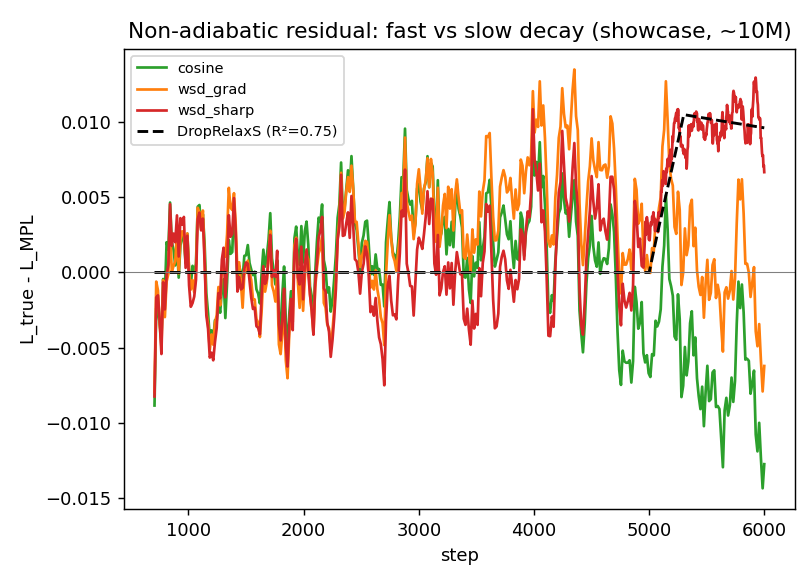
\includegraphics[width=0.96\linewidth]{figs/fig_real_transformer.png}\\[2pt]
\textbf{从零 AdamW 量化确认:} $\tau\propto1/\eta$ \hl{$p=0.971$}、$\beta_2$ 无关 \hl{CV 1.1\%}、
\hl{幅度恒等 $dL_{\rm eq}/d\eta=3.075$ vs 闭式 $3.0$(<3\%)}。可证伪。
\end{column}
\end{columns}
\vfill
{\footnotesize\textit{诚实标注:~10M 上 $\tau\propto1/\eta$ 未解析($\tau$ 平,审计确认非窗口伪影);
单曲线上核与绝热基线简并——与论文"数据稀缺、领头阶"的适用范围一致。}}
\end{frame}

% =====================================================================
\section{结论}
\begin{frame}{结论}
\textbf{我们做了什么(覆盖 Task 2 三要素)。}
\begin{itemize}
  \item \hl{问题}:调度感知损失曲线预测,cosine$\to$WSD。
  \item \hl{复现}:忠实重现 Tissue \& MPL,对齐已发表精度。
  \item \hl{方法开发}:指出现有律皆为\emph{绝热},推导并验证其首个\emph{非绝热}修正。
\end{itemize}
\textbf{核心贡献。}
\begin{itemize}
  \item 绝热/非绝热分解:损失不仅依赖"花了多少 LR",还依赖"花得多快";
  \item 从 AdamW 预条件动力学\emph{推出} $\Drop$,幅度 $=dL_{\rm eq}/d\eta$(精确恒等式);
  \item 推出并\emph{实测确认} $\tau\propto1/\eta$($p=1.00\pm0.18$),自洽验证噪声主导;
  \item 形状常数尺度不变 $\Rightarrow$ \hl{参数无关跨尺度预测,陡降 $-44\%$、胜 6/6}。
\end{itemize}
\textbf{局限。} 增益限于数据稀缺的陡降;$\lambda_{\rm slow},c$ 是测的非算的;单一公开数据集、三尺度;
有限 $\beta_2$ 第二通道待验证。
\end{frame}

\begin{frame}{可复现性}
\begin{center}\small
\begin{tabular}{ll}
\toprule
结果 & 命令 \\
\midrule
复现(表 1) & \texttt{repro/reproduce\_cosine\_to\_wsd.py}\\
残差 $=\Drop$、R² & \texttt{repro/nonadiabatic\_theory.py}、\texttt{deep\_stime2.py}\\
$\tau\propto1/\eta$($p{=}1.00\pm0.18$) & \texttt{repro/deep\_tau.py}\\
S-时间核、$\lambda_{\rm slow}$ 扫描 & \texttt{repro/deep\_stime.py}\\
谱混合(双指数)与自洽性 & \texttt{repro/deep\_rigor.py}\\
\hl{参数无关跨尺度预测 $-44\%$} & \texttt{repro/deep\_predict.py}\\
公平基线(信息 vs 公式缺口) & \texttt{repro/correction\_fair.py}\\
推导文档 & \texttt{docs/core/nonadiabatic\_correction.md}\\
\bottomrule
\end{tabular}
\end{center}
\vfill
\centering\footnotesize
\texttt{pip install -r requirements.txt};数据:官方 MPL 公开曲线,随仓库置于
\texttt{external/MultiPowerLaw/}。
\end{frame}

\begin{frame}{分工与致谢}
\textbf{团队。} 单人组:\textbf{吴家驹}(2400010711,本科生)—— 全部工作(复现、推导、实验、写作)
由唯一作者完成。
\vfill
\textbf{资源与参考。} 数据:官方 Multi-Power-Law 公开损失曲线($25/100/400$M $\times\ 9$ 调度)。
主要参考:Tissue et al.\ (2024);Luo et al.\ (2025, MPL);Li, Chen, Huang, Wang \& Wu
(2025, FSL);Cohen et al.\ (2021/22, edge of stability / Adam);Wen et al.\ (2024, river valley)。
\vfill
\centering\small 代码与文档:\texttt{github.com/wjjpku/DL-final}
\vfill
\centering\Large 谢谢！\quad\normalsize 欢迎提问。
\end{frame}

\end{document}
